\documentclass{article}

\usepackage{times}
\usepackage{geometry}
\geometry{a4paper,left=0.6cm,right=0.7cm,top=1cm,bottom=1cm,columnsep=0.8cm}

\usepackage{fontawesome}
\usepackage[hidelinks]{hyperref}
\usepackage{multicol,paracol,tikz,hyphsubst,moresize,hyphenat,adjustbox,tabularx,xcolor,enumitem}
\newcolumntype{Y}{>{\RaggedRight\arraybackslash}X}
\setlist[itemize]{itemsep=1pt,leftmargin=*,topsep=-10pt}

\definecolor{maincolor}{HTML}{ffffff}
\definecolor{seccolor}{HTML}{0b1f3b}
\definecolor{gray}{HTML}{8c94a9}
\definecolor{sidetext}{HTML}{59cee5}
\definecolor{Green}{HTML}{2caf00}
\definecolor{lightgray}{HTML}{D3D3D3}

% --- bande latérale bleue
\usepackage{eso-pic}
\AddToShipoutPictureBG{%
  \begin{tikzpicture}[remember picture,overlay]
    \fill[seccolor] (0.7\paperwidth,0) rectangle (\paperwidth,\paperheight);
    \fill[maincolor] (0,0) rectangle (0.7\paperwidth,\paperheight);
  \end{tikzpicture}%
}

\setlength{\parindent}{0pt}
\newcommand{\cvsection}[1]{%
  \par\bigskip                % espace avant le titre
  {\bfseries\Large #1}\par
  \noindent\rule{\linewidth}{0.8pt}\par
  \medskip                    % espace après la ligne
}

\newcommand*{\ClipSep}{0.4cm}

% ------------------------------------------------------------------
\begin{document}\pagestyle{empty}
\columnratio{0.7}\begin{paracol}{2}

% --------- colonne gauche -----------------------------------------
\begin{minipage}{0.7\linewidth}
{\LARGE\textbf{Pape Saliou FALL}}

\bigskip
{\large\textbf{Ingénieur Data Scientist \& Développeur IA}}
\end{minipage}\hfill
\begin{minipage}{0.18\linewidth}
\begin{tikzpicture}
\node[inner sep=0pt]{ 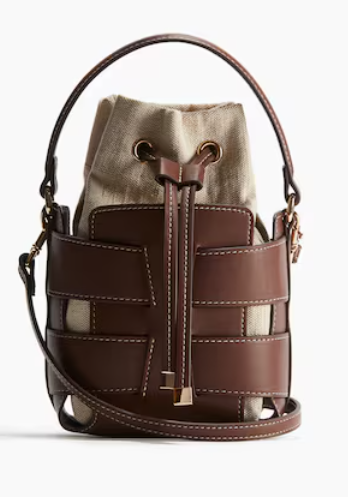
\includegraphics[width=\linewidth]{7617401e87354f10be0ed128ec4c0189.png} };
\draw[white,rounded corners=\ClipSep,line width=\ClipSep]
      (current bounding box.north west) --
      (current bounding box.north east) --
      (current bounding box.south east) --
      (current bounding box.south west) -- cycle;
\end{tikzpicture}
\end{minipage}

\cvsection{Profil}
Data Scientist confirmé, je conçois et déploie des solutions d’intelligence artificielle transformant des données complexes en leviers de performance. Autonome et force de proposition, j’orchestre l’ensemble du cycle de vie data : collecte, modélisation, industrialisation et mise en production. Passionné par l’innovation, j’évolue aisément dans des environnements agiles et collaboratifs, où je mets la valeur métier au cœur de chaque projet.

\cvsection{EXPÉRIENCE}

\colorbox{maincolor}{%
  \begin{minipage}{\linewidth}
    \textbf{Data Scientist \& Développeur IA} \\ Prepaya \\ Depuis 01.2024
    \begin{itemize}
      \item Développé une plateforme IA full-stack (Python/JavaScript) déployée sur Heroku, facilitant l’accès aux modèles prédictifs pour les équipes métiers. \item Implémenté des algorithmes de Machine \& Deep Learning (scikit-learn, TensorFlow, Keras) pour l’analyse de séries chronologiques et données clients, améliorant la précision des prévisions. \item Créé une API OpenAI et intégré PostgreSQL afin de sécuriser et industrialiser l’usage des fonctionnalités d’IA.
    \end{itemize}
  \end{minipage}}

\vspace{3mm}


\colorbox{maincolor}{%
  \begin{minipage}{\linewidth}
    \textbf{Apprenti Risk Analyst \& Data Scientist} \\ AXA XL \\ 12.2022 - 12.2023
    \begin{itemize}
      \item Automatisé la collecte de données financières via scripts Python/VBA, réduisant de 60 \% le temps de préparation des rapports. \item Conçu des tableaux de bord Power BI pour le suivi de facturation et KPI financiers, offrant une visibilité temps réel au management. \item Développé un modèle de prédiction de sinistres (Python, R Shiny) améliorant la détection des risques et la prise de décision.
    \end{itemize}
  \end{minipage}}

\vspace{3mm}


\colorbox{maincolor}{%
  \begin{minipage}{\linewidth}
    \textbf{Apprenti Data Scientist} \\ Prepaya \\ 09.2021 - 08.2022
    \begin{itemize}
      \item Appliqué des techniques de Deep Learning NLP (T5, BERT) pour générer automatiquement des formulaires, réduisant la saisie manuelle. \item Réalisé une analyse de sentiments sur les retours clients afin d’identifier les axes d’amélioration produit. \item Industrialisé les pipelines de web scraping et de traitement de texte (BeautifulSoup, Selenium, PyTorch) dans un environnement Python.
    \end{itemize}
  \end{minipage}}

\cvsection{FORMATION}

    \begin{tabularx}{\linewidth}{@{}c X@{}}
    \textcolor{sidetext}{\faGraduationCap} &
    \textbf{Master 2 Data Science} \\
    & Sorbonne Université, Paris \\
    & \begin{itemize}[leftmargin=*]
  \item Cours avancés d’analyse de données, machine et deep learning. \item Approfondissement des modèles statistiques, séries chronologiques et calcul parallèle.
\end{itemize} \\
    & \textit{09.2021 - 03.2022}
    \end{tabularx}
    

% --------- colonne droite (bleue) ---------------------------------
\switchcolumn\color{white}\hspace*{0.4cm}\begin{minipage}{0.88\linewidth}

\cvsection{CONTACT}
\begin{tabular}{@{}c l}
  \faPhone & \href{tel:07 53 48 14 53}{07 53 48 14 53} \\[2pt]
  \faEnvelope & \href{mailto:papesalioufall2@gmail.com}{papesalioufall2@gmail.com} \\[2pt]
  \faMapMarker & 95300 Pontoise\\ \\[2pt]
  \faLinkedin & \href{https://www.linkedin.com/in/pape-saliou-fall-43154a211}{pape-saliou-fall-43154a211}
\end{tabular}

\cvsection{COMPÉTENCES}

\begin{itemize}[leftmargin=*]
\item Python
\item JavaScript
\item C
\item C++
\item R
\item SQL
\item PowerBI\end{itemize}
\par\bigskip 

\cvsection{LANGUES}
\begin{itemize}[leftmargin=*]
\item Français - \textcolor{gray}{Maternel}
\item Anglais - \textcolor{gray}{B2}\end{itemize}
\par\bigskip 
\cvsection{INTÉRÊTS}
\begin{itemize}[leftmargin=*]
\item Football
\item Natation
\item Lecture
\end{itemize}

\end{minipage}
\end{paracol}
\end{document}
